\paragraph*{}
The first step of the implementation was to pick our \quotes{\emph{arsenal}}, i.e. the set of readily available agents that we would use as our set of strategies. We used participants in the \href{https://web.tuat.ac.jp/~katfuji/ANAC2022/}{2022 ANAC competition} \cite{ANAC}, selected through a process described below. We chose to implement a neural network (NN), trained to find correlation between domain characteristics and agent performance to estimate how well those agents would do in a new domain. We also chose to model the competition as a Multi-Armed Bandit (MAB) setting and implement a modified version of the Upper Confidence Bound (UCB) algorithm to keep learning during the competition while keeping performance as our primary objective.

\paragraph*{}
In \cref{fig:high_level_overview} we present the process followed by our agent when asked to participate in a new negotiation session. Observe the distinction between new domains (meaning we have not negotiated in them) and domains we know something about: 
\begin{itemize}
    \item In a new domain (one we have not negotiated in before), we feed its characteristics (see \quotes{features} \hyperref[list:features]{\underline{\emph{below}}}) to the neural network, which outputs an estimate for the performance of each agent in our arsenal. We then use those estimates to initialize our UCB machinery, which ultimately tells us which strategy we should employ in the upcoming session.
    
    % TODO: kapou na peis kai oti to ucb einai pio xrhsimo otan exeis perissoterous antipalous giati paizeis pio polles fores sto idio domain opote ksereis kalytera ti doulevei ekei. sovaro limitation to oti den diaforopoiesi me vash antipalo, alla nai. we could say that it tends to average out over many opponents (since encountering a hardliner for example is equally frequent with encountering a conceider (greedy - non greedy if you will) - which is not really the case, since noone would submit a conceider in a general purpose tournament but yeah.) 
    \item If we have already encountered the domain we are about to negotiate in, the process above has already taken place, so we do not need to use the NN. We feed the pre-existing estimates to the UCB machinery that once again picks the best available strategy.
\end{itemize}
In both cases, right after the session ends, we check the utility that its result gave us and feed it to UCB in order to adjust our estimate for the picked strategy. That way we can adapt to the environment, by not just trusting the NN's estimates, but rather observing reality and adjusting our beliefs accordingly.

\begin{figure}[H]
\centering
\framebox{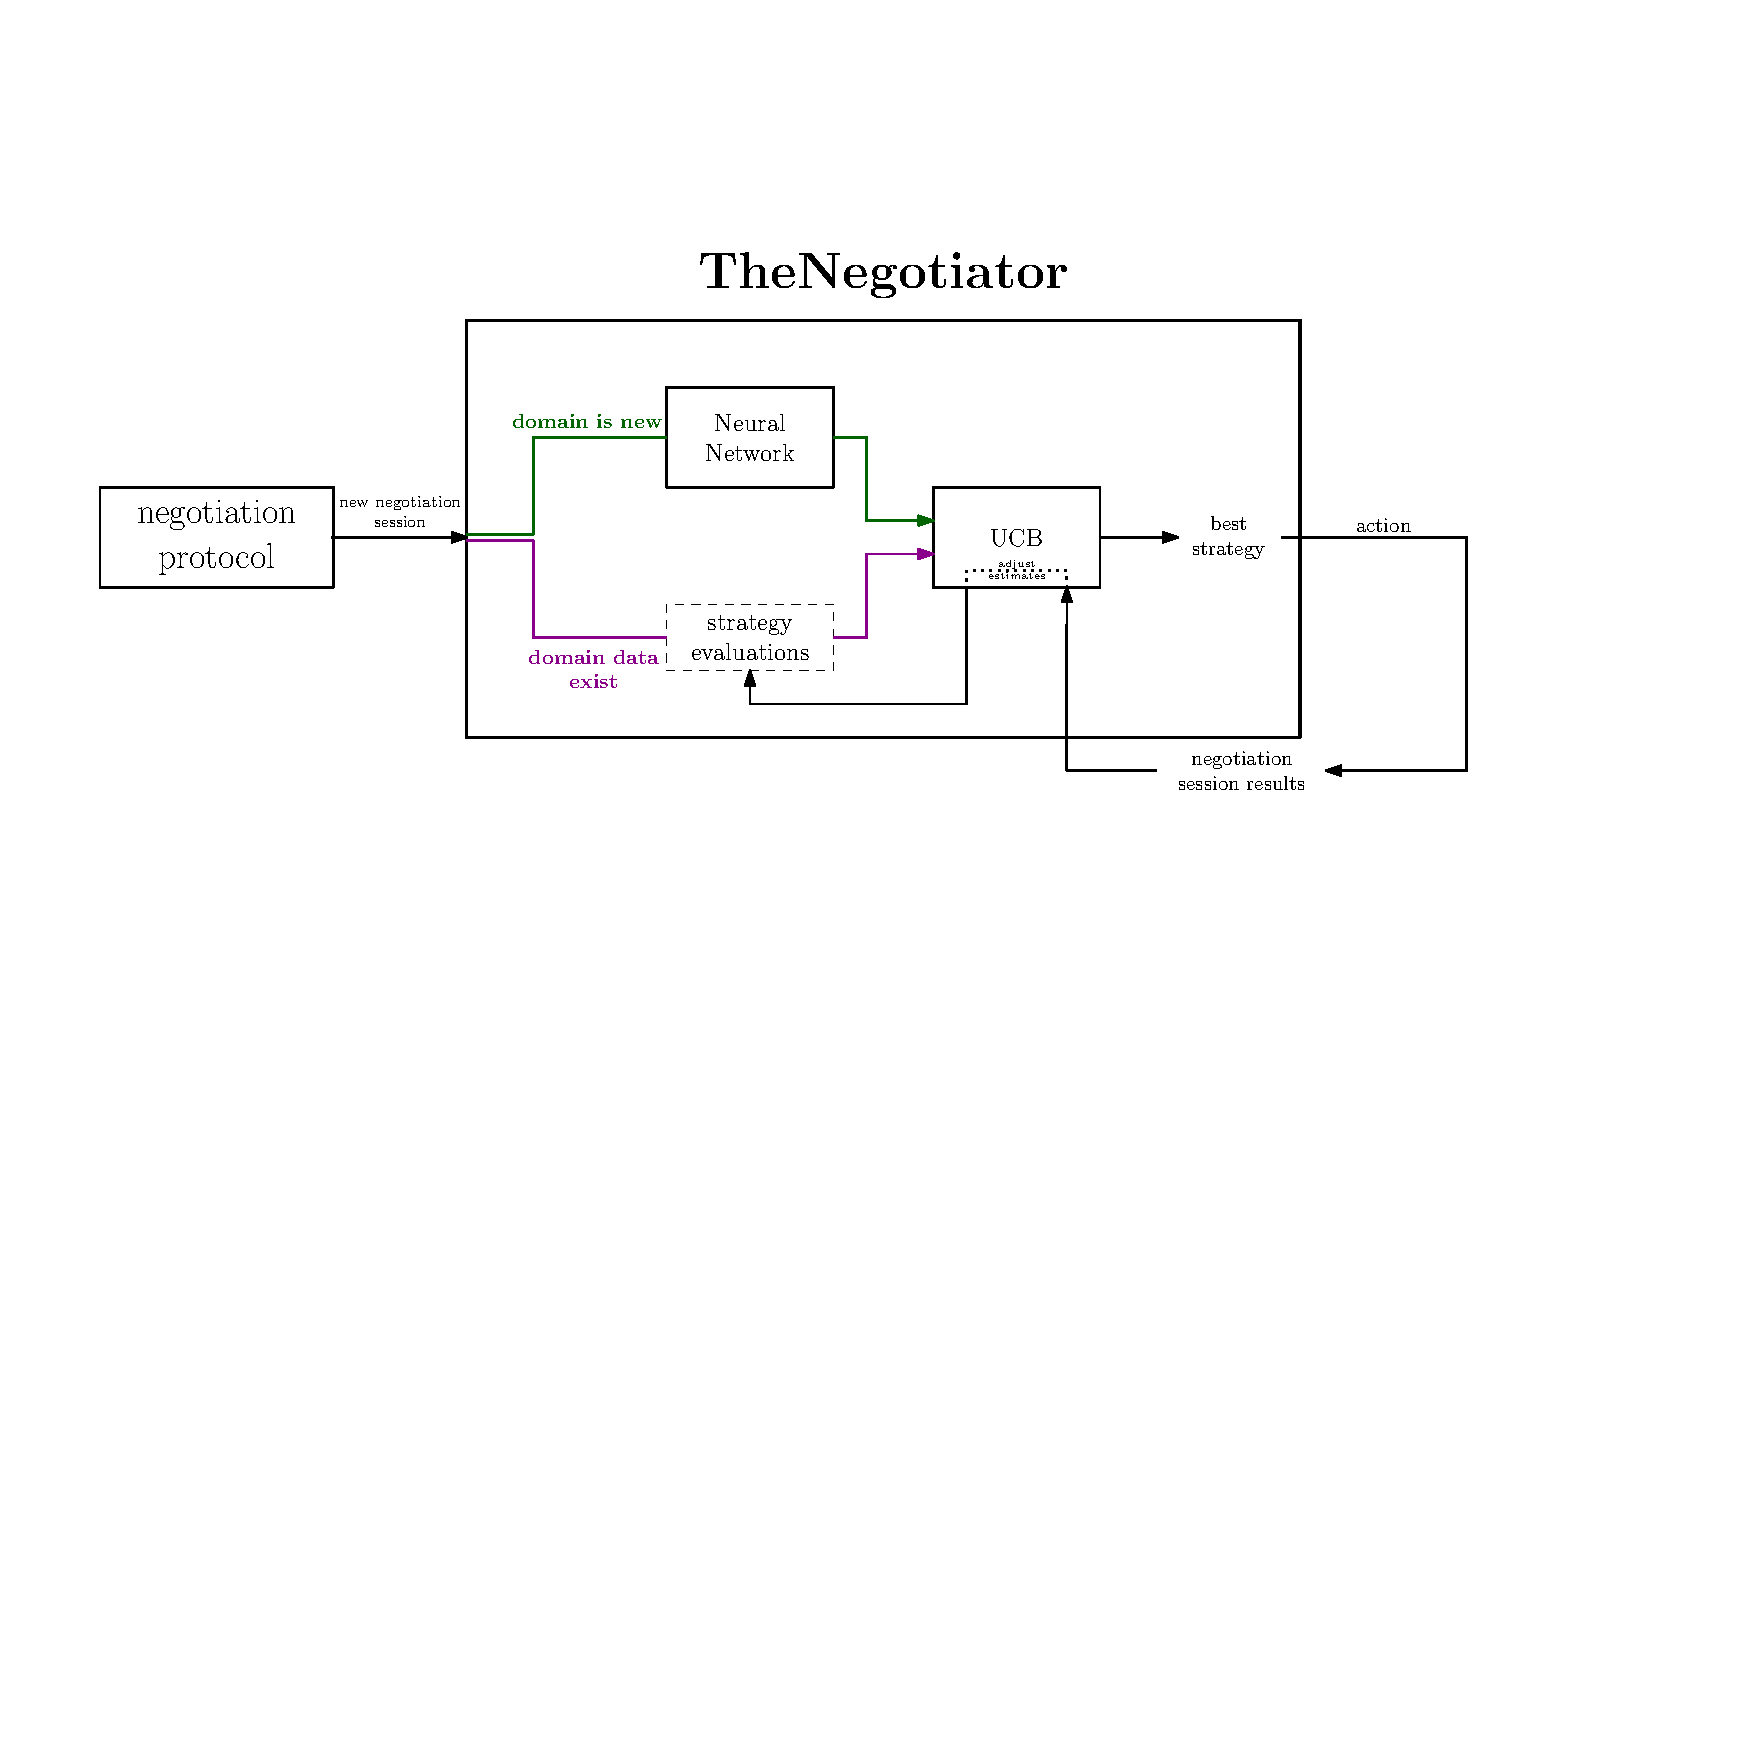
\includegraphics[scale=0.5]{high_level_overview.pdf}}
\captionsetup{justification=centering}
\caption{A high-level overview of TheNegotiator's function}
\label{fig:high_level_overview}
\end{figure}
